%!TEX root = ../Report.tex

In this chapter, we cover the current approaches to parallel programming. We then explore the key ideas requisite to this project, in order to discuss how they are combined and their implications. Finally, we review what was done in the previous year of this project \cite{me}, and some of the lessons we carried forward to this year.

\section{Introduction}
\label{section:background:introduction}

The three pertinent ideas to this project are those of plasticity, contention aware scheduling, and skeleton programming. We briefly cover these here, and provide more detailed explanations later.

A plastic program is a program which can adapt to its current environment. For example, a program may utilise plasticity in order to alter its operations to suit a particular architecture. In our case, the program will alter its implementation in response to the current state of the system, with a focus on which other programs may be active.

Contention aware scheduling is the idea of taking into account possible contention when scheduling programs, and is particularly relevant when considering machines with multiple sockets. We may know that certain programs run well together, and so we would schedule them to run together on the same socket. Similarly, we would try to keep more contentious programs apart, running on separate sockets.

Skeleton programming involves the use of an algorithmic skeleton. The skeleton provides the outline of the algorithm, and the user supplies some code to produce a complete program. With skeletons for common programming patterns, these are particularly useful for parallel programming, as they abstract away complexity, making producing correct and efficient parallel programs easy.

The overall aim of this project is to investigate if we can gain performance by utilising all of these ideas with parallel programming. 



\section{Parallel Programming}
\label{section:background:parallel_programming}

Writing correct parallel programs is hard \cite{parallel_hard}. It introduces new difficulties such as race conditions and thread safety. Writing efficient parallel applications, where performance matters, is even harder \cite{parallel_hard_perf}. The overhead of parallelism must be kept small enough such that any performance gains will outweigh it. 

Current solutions range from providing the programmer with low level primitives (POSIX Threads \cite{posix_threads}), to abstracting away these primitives, resulting in a higher level language (OpenMP \cite{openmp}). Other solutions focus on making parallel programming easier, usually employing skeleton code (Intel Threaded Building Blocks \cite{threading_building_blocks_2018}).

In this project, we are combining the ideas of plasticity and contention aware scheduling with parallel programming, with a focus on efficiency. This, along with the difficulty of parallel programming, makes it hard to ensure correctness, and particularly efficiency. Since the goals of this project will require the cooperation of several programs, it is in our interest to make using these techniques as easy as possible, to encourage their use by programmers. Thus, to abstract this complexity away from the programmer, we employ skeletal programming. This also has the beneficial side effect of dividing the challenge into a pattern-by-pattern basis. 



\subsection{Current Solutions}
\label{section:background:current_solutions}

Since we are investigating the feasibility of a new parallel programming library, it is worth giving a quick overview of some current parallel programming solutions. These include:

\begin{itemize}
	\item Pthreads (POSIX Threads \cite{posix_threads})
	\item MPI 	   (Message Passing Interface \cite{mpi})
	\item OpenMP   (Open Multi-Processing \cite{openmp_home} \cite{openmp})
	\item Intel\textsuperscript{\textregistered} TBB (Intel Threading Building Blocks \cite{threading_building_blocks_2018} \cite{contreras_martonosi_2008})
	\item SkePU (\cite{skepu} \cite{skepu_2_2018})
\end{itemize}

Pthreads and MPI represent the most direct methods of parallel programming, whereas OpenMP, Intel TBB, and SkePU focus on making parallel programming simpler. 

\begin{description}
\item[Pthreads] is a set of interfaces (functions, header files) for multi-threaded programming. A process can contain multiple threads, all of which collaborate on the same program. It is targeted towards shared memory architectures, so threads share global memory (data and heap), but each thread has its own stack (automatic variables). The low level nature and the portability of Pthreads makes it suitable for building other parallel programming mechanisms.

\item[MPI] is a message passing standard, and as such it describes how processes can communicate. The message passing model is attractive because it provides portability, and it can be used for communication in both distributed or shared memory systems, networks of computers, or any combination of these. Its versatility and efficiency allows for portable and scalable parallel programs, and as a result, it is the dominant model used in the high performance computing industry today \cite{mpi}. 

\item[OpenMP] is an API which supports shared memory multiprocessing programming in C, C++, and Fortran. It consists of compiler directives, library routines, and environment variables. Like Pthreads, OpenMP is intended for shared memory architecture, however it abstracts away many of the primitives which are present in Pthreads. As such it provides a simple and flexible interface, whilst also being portable and scalable. 

The approach taken with some computer clusters is a mix of both OpenMP and MPI, such that OpenMP is used for parallelism within a node while MPI is used for parallelism between nodes. The main benefit of this is reduced communication bandwidth \cite{mixed_openmp_mpi}.

\item[Intel TBB] is a C++ template library developed by Intel for parallel programming on multi-core processors. It breaks down computations into tasks, constructing dependency graphs according to algorithmic skeletons (described in section \ref{section:background:what_is_skeleton_programming}). The library then schedules threads to execute these tasks, respecting the dependencies.

Designed to make parallel programs easier to write, it has the advantage of low-overhead polymorphism, since templates are a compile-time construct, meaning there is little loss in performance compared to hand written programs, provided your application can be described using the templates.

\item[SkePU] is an open-source skeleton programming framework for multicore CPUs and multi-GPU systems. It is a C++ template library with data-parallel and task-parallel skeletons, and support for execution on multi-GPU systems both with CUDA and OpenCL.

Similar to Intel TBB, it attempts to simplify parallel programming through the use of templates (here called skeletons). However, SkePU adds features such as multiple back ends, including OpenMP, OpenCL, CUDA, and multi-GPU OpenCL and CUDA. It also provides a tuning framework for context-aware implementation selection, allowing it to select the expected fastest implementation at each skeleton call. This differs from our system in that it performs static analysis before the program is run, and as such it cannot react to changes in the system at runtime. It also does not utilise plasticity at a more fine grained level than which language (or hardware) to use.
\end{description}



Parallel programming introduces a whole host of complications ranging from race conditions to limited scalability. These new problems can certainly be overwhelming to a traditionally sequential application programmer, so much so that there are entire books dedicated to the use of parallel programming methods. Given that this is already so hard, and we require plasticity on top of this, we must simplify what we present to the programmer, otherwise it would be too formidable. Like Intel TBB and SkePU, we do this by utilising skeletons/templates.



\section{What Is Contention Aware Scheduling?}
\label{section:background:what_is_contention_aware_scheduling}

We use contention aware scheduling as a means to address a particular problem. In our case, the problem is that programs running simultaneously on the same machine will interfere with each other, as they must compete for resources. This interference is not uniform (as can be seen in figure \ref{fig:lira_pairwise_speedup}), and, in fact, is dependent upon which programs are running, as well as the overall state of the system. Contention aware scheduling is the practice of taking into account this interference (contention) when scheduling programs, such that programs which work well together are scheduled to run on the same socket, thus reducing the overall contention.

LIRA \cite{lira} shows that throughput gains of 3-7\% can be seen with this technique. Extending this with plasticity would mean that we can control which program runs where, and the implementation each program uses, allowing us more scope to mitigate contention.

\begin{figure}[H]
	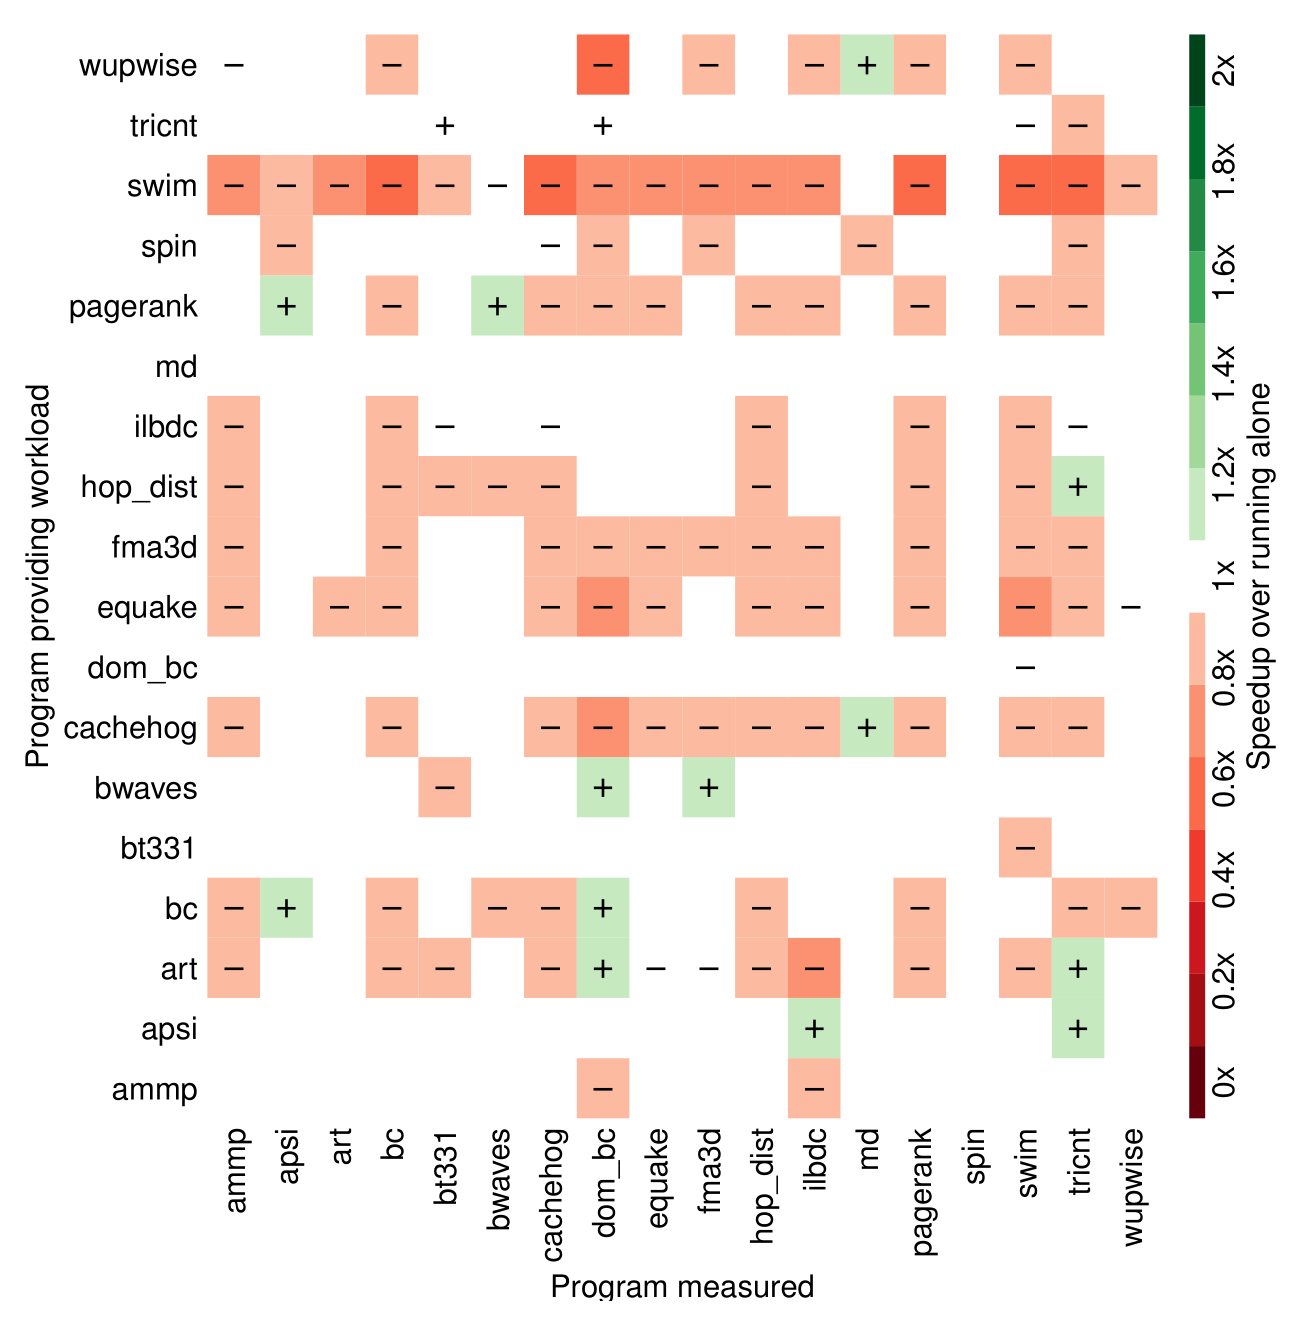
\includegraphics[width=\textwidth]{graphics/lira_pairwise_speedup.png}
	\caption{Taken from the LIRA paper \cite{lira}: Pair-wise speedup of programs, comparing sharing a socket to running in isolation. Boxes annotated with a $-$ indicates where performance decreased when sharing a socket, and $+$ shows increases. For example, looking at the programs bc and swim, we see a speedup of around 0.6x, whereas for the programs apsi and pagerank, we see a speedup of around 1.2x.}
	\label{fig:lira_pairwise_speedup}
\end{figure}





\section{What Is Plastic Programming?}
\label{section:background:what_is_plastic_programming}

When programming an algorithm, there are often choices which can greatly affect performance, and the optimal choice depends on the circumstances. As an example, for a sorting problem with a large input size, radix sort would perform best. For a small input size, insertion sort would be better. Parallel programs tend to have more choices, particularly with a view to keeping overhead reasonable.

Plastic programming is the idea of a program which includes multiple implementations, which can be chosen between dynamically. The mechanism for selecting the implementation can vary, back with our sorting example, we could assess the input size, and run radix sort until the problem is small enough to use insertion sort. Figure \ref{fig:plastic_graph} illustrates such a situation.

\begin{figure}[H]
	\centering
	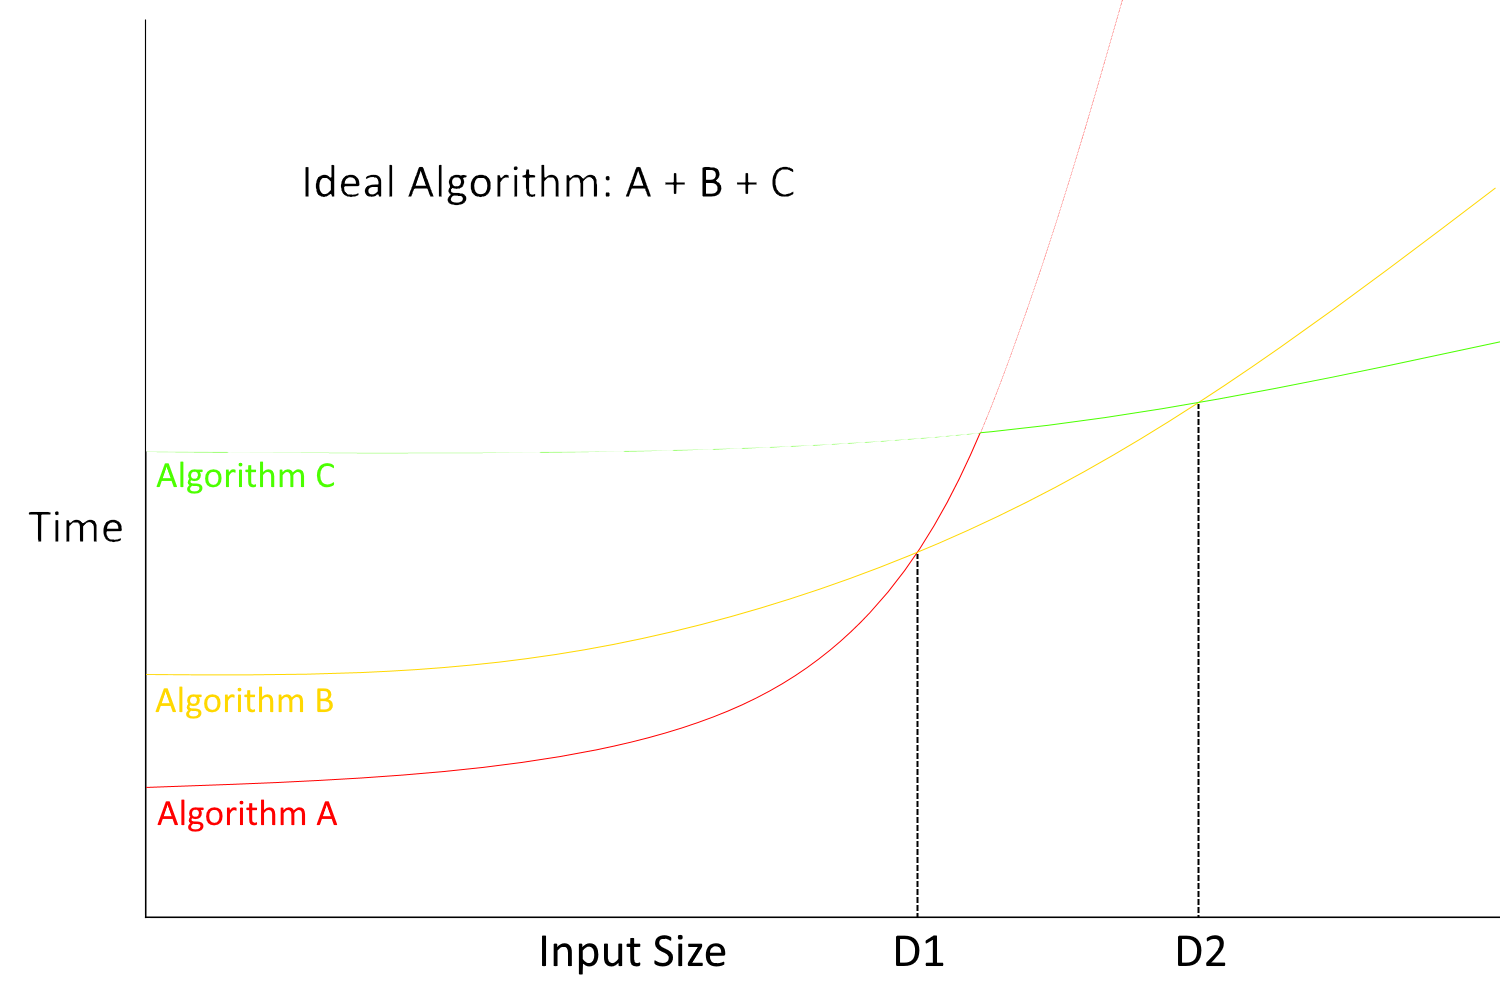
\includegraphics[width=\textwidth]{plastic_graph}
	\caption{A graph showing three algorithms with different runtime curves, which depend upon the array size. Combining these algorithms would provide an improved algorithm, with D1 and D2 showing optimal decision points where a plastic programming system should switch algorithms}
	\label{fig:plastic_graph}
\end{figure}



\section{What Is Skeleton Programming?}
\label{section:background:what_is_skeleton_programming}

Skeleton programming is a high-level programming model, which will allow us to abstract away the details of parallel programming, plastic programming, and contention aware scheduling. The idea is that the skeleton provides the core structure of an algorithm, with the user providing some code, producing a correct and hopefully efficient program \cite{patterns_and_frameworks}. Multiple skeletons can be combined to produce a more complex program, for example map and reduce skeletons are commonly combined. This makes skeletons powerful tools for easily creating clean, complex programs.

This makes using our library much easier, and means that we can assess the program's complexity, since we know the algorithmic details of the skeleton.



\section{Review of Previous Year}
\label{section:background:review_of_previous_year}

The main goal of this two year project is to investigate if we can gain some extra performance in parallel multi-programming systems by exploiting contention aware scheduling and plastic programming. We are not aware of any published previous work on runtime dynamic plastic parallel skeletons, as described in this project.

In the first year of this project \cite{me}, we investigated a basic parallel programming pattern, map-array. We incorporated this into a feasible estimate of a contention aware plastic parallel programming library, and measured the performance, with a focus on understanding and minimising overhead. In this section, we cover the design of this library, and the information gained from its analysis.


\subsubsection{Design}
\label{section:background:design}

In order to make such a library, we needed to make two modifications to a typical parallel program. We needed to add plasticity to the program itself, and to introduce some form of communication and synchronisation with other programs running in the system. This synchronisation could be distributed, or centralised. For the initial investigation, we decided that centralised was more appropriate to keep things simple.

\begin{itemize}
    \item Plasticity
    
        To implement plasticity, we added the ability to vary three key aspects of the implementation of a single instance of the map-array skeleton:
    
        \begin{itemize}
        	\item Thread count - The number of threads we split the tasks between
        	\item Thread pinnings - The particular CPU cores each thread could utilise
        	\item Schedule - How we divided tasks between threads
        \end{itemize}
        
        These were set before any worker threads were spawned. This allowed us to generate several different implementations by altering these parameters.
        
        However, this alone did not allow us to dynamically switch implementations during runtime. The simplest way to make this dynamic would be to gracefully kill all worker threads, and restart them with the new parameters. We chose this method to, again, keep it simple. The cost incurred (closing and restarting each thread) would be proportional to how often we want to change parameters, and as such, its overall impact depended upon the frequency of change. We also investigated the impact this method had, finding it to be negligible.
    
    \item Communication
    
        As discussed previously, we decided upon the use of a centralised controller program, which would communicate with each application running an instance of our library and instruct them what parameters to use.
        
        When a new instance of the library started, it registered with the controller program. The controller then continually monitored the system for any changes, and reacted accordingly sending new parameters to each registered program. For our purposes, the controller acted according to a predefined set of instructions, telling it what parameters to send and when. In a more developed system, the controller would monitor the system and send updates programmatically.
        
        To allow instances of our library to communicate with the controller, we added a ``main'' thread, to handle communication operations, and update the worker threads with new parameters. This communication structure is illustrated in figure \ref{fig:old_communication_structure}.
        
        \begin{figure}[H]
            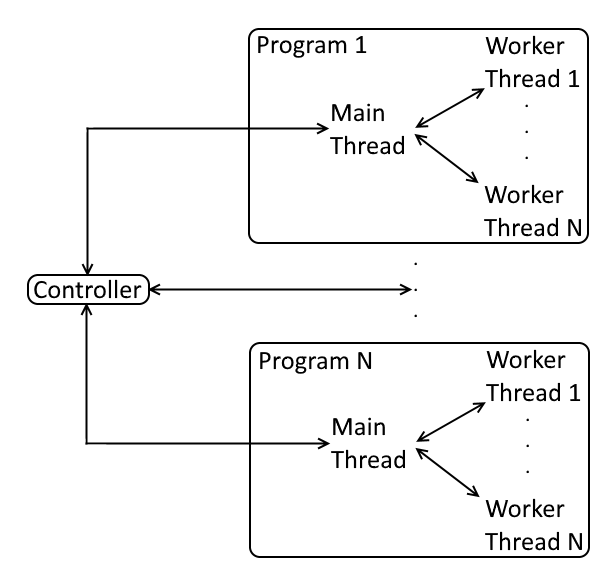
\includegraphics[width=1\textwidth]{graphics/communication_structure.png}
            \caption{A high level communication model of the system, with an arbitrary number of programs, each with an arbitrary number of threads. Two way communication occurs between the controller and each main thread, and then between each main thread and its worker threads.}
            \label{fig:old_communication_structure}
        \end{figure}
\end{itemize}



\subsubsection{Results}
\label{section:background:results}

The two aims of the project work from the previous year were:

\begin{itemize}
    \item Assess the feasibility and the overhead introduced by a contention aware plastic parallel programming library
    
    \item Assess the potential performance gains to be had by extending contention aware scheduling with plasticity
\end{itemize}

Regarding the first item, we found that while programming the library was complex, using it was straight forward, as expected. As for the overhead, compared to running the programs with hand coded solutions, we found it acceptable. Thus, it is feasible if we see reasonable gains from adding plasticity to contention aware scheduling, that the overhead could be amortised.

For the second item, we found that whilst the results were promising, the map-array pattern was limited in the performance gains to be had from plasticity.



\subsubsection{Lessons to be Carried Forward}
\label{section:background:lessons_to_be_carried_forward}

The performance results of the previous year showed promise, but further exploration was required, which is our focus this year. We saw some gain in certain circumstances, but we concluded that the map array pattern used was too predictable, and that it didn't have have much scope for plastic improvement. However, it would still be reasonable to use our library for map array patterns, since other programs on the system may benefit.

This issue is why we decided to focus on the stencil code pattern this year, as it is much more complex to parallelise, with more scope for our decisions to have an impact.